\chapter{Electrophoresis and Charge Screening in Fluids}
\thispagestyle{fancy}
\fancyhead[RE,LO]{Experiment \thechapter}
%
The biophysical motivation for this laboratory is the ubiquity of charges in living systems.
Large molecules—in particular, proteins—are often phosphorylated and thus carry net charge.
These charges generate electric fields, exerting attractive forces on other molecules, and playing a role in the intricate balance of forces and movements that occur in a living cell!
We might ask: how far is the reach of the force field from a charge in a large protein when many ions are present in the surrounding fluid?
How fast would a charged protein move in an electric field?
These effects are crucial for understanding biological systems at the cellular level.
\par 
In this experiment, we will investigate related questions in a simple model system.
You will be investigating charge screening in fluids by employing the technique of electrophoresis.
Your investigation will come in two parts: an investigation of glass beads in de-ionized water (DI water, pure H$_{2}$O), and an investigation of glass beads in two saline solutions of different concentrations.
\par 
%We have been employing solutions of glass beads in water in most of our labs.
You may notice that some of the beads are stuck together, forming clumps (also called `flocs' because their aggregation (coming together) is a form of `flocculation'), or that the beads sometimes ``settle-out'' of the fluid (like the sedimentation we observed in the tilted microscope lab last semester). 
Aggregation (flocculation or coagulation) and sedimentation are behaviors common to colloidal fluids. 
A colloidal system is one in which one phase of matter is finely dispersed throughout another phase of mater. 
Our glass beads in water are colloidal fluids because the glass beads (solids) are small particles dispersed throughout the water (fluid). 
\par 
When the glass beads are submerged in water, they become charged — even in DI water! 
The glass beads, SiO$_{2}$, have surface groups of SiOH. 
When immersed in water, the hydrogen nucleus breaks free (increasing the acidity of the fluid due to the roaming H$^{+}$) and leaving an SiO$^{-}$ behind. 
Thus the surface of the glass beads becomes negatively charged — each bead carries charge on the order of femto-Coulombs (fC). 
(Lest you think a fC is small, about how many extra electrons are on each bead?) 
[You might then ask, if all the beads are negatively charged, then why do they stick together? 
Besides the electric repulsive forces between the beads, there are also attractive van der Waals forces; at close enough distances, the attraction dominates the interaction and the beads will stick together to form a floc.] 
If a salt (like NaCl) is added to the fluid, it will dissolve and the free cations (or anions, for a positively charged colloid) will group around the negatively charged beads of glass, thus decreasing the `effective charge' of the unit — this is called `charge screening' or `Debye screening.' 
The more ions that are available in the fluid, the greater the charge screening effect will be; thus the concentration of the electrolyte is important.
\par 
We can investigate these charges using the technique of electrophoresis. 
By applying an electric field (generated by a potential difference between two electrodes) to the fluid, we can cause an electric force on the charged beads that will induce motion through the still fluid.
A larger electric field will cause faster motion. 

\paragraph{For this two week lab:} Your overall task for the next two weeks is to determine how charged our glass beads are in DI water and then compare that charge to the `effective charge' as seen in various concentrations of saline solution.
You will do this in multiple stages:
\begin{enumerate}
\itemsep-0.2em
\item Create a model of the forces acting on your beads in a solution.
\item Discuss as a class what you need to measure, and how you will calculate the charge on your beads.
\item Capture your first video according to table~\ref{tab:lab7-vids} and analyze it. Make sure that the surface charge values that you calculate make sense.
\item Collect the rest of your videos and analyze them.
\end{enumerate}

\section{Modeling Electrophoresis}
Before you begin taking data, you will need to model the situation: consider what forces act on the bead as it moves through the fluid and determine how changing the potential difference between the electrodes and measuring the resultant speed of the beads will enable you to find the charge on the beads. 
Carefully reflect on what assumptions you are making as you model the situation and think about the implications these assumptions have for the design of your experiment.
\par 
After modeling the situation, design an experiment to determine the charging of beads in fluid. 
Consider 'broad stroke' details (e.g., What data are we collecting? How much data is 'enough'?) as well as 'fine stroke' details (e.g., What part of the slide are we viewing? How are we collecting data? How do our assumptions affect our procedure and analysis?). 
Be sure to consider the qualitative aspects of the motion, as well (e.g., Is this really directed motion? Could it be random motion? Which electrode (+ or -) are the beads moving toward?). 
Once you have a good experimental design, gather data to determine the charging of our glass beads in DI water.

\section{Measuring Electrophoresis}
For this experiment, you will be using a microscope to observe the motion of aqueous micropheres within an electric filed. If you are unfamiliar with how to operate a microscope, including how to capture video using one, please read through Technical~Document~\ref{chap:scope-basic}. The experimental set-up available includes:
\begin{itemize}
\itemsep-0.3em
\item Microscope with camera.
\item Power source to create constant voltage of your choosing
\item Two wires with banana plugs on one end and alligator clips on the other (for holding electrodes, see figure~\ref{fig:electroph})
\item Short segments of copper wire to use as electrodes
\item A 24 well plate (fill one of these chambers with enough solution to cover the bottom for each investigation — when investigating a different solution, you can simply move to another chamber. At the end of the the first day, please put your name on your chamber slide and store in the cabinet. Each well has a diameter of 15.5 mm.)
\item Three vials of solution: one of distilled water and two different saline solutions (LOW and HIGH)
\item Other tools (rulers, paper towels, pipettes, etc.)
\end{itemize}

\noindent
If you have never used a power source before, ask your TA for safety and use instructions. Here are some other details that may help you while performing your experiment:

\begin{itemize}
\itemsep-0.3em
\item The maximum voltage the power source can produce is 18 V; you will likely need 4 V or more to see bead motion in DI water.
\item The wells each need less than 1 mL of fluid to coat the bottom; the vials provided should be sufficient.
\item You should gather your video data as soon after applying the potential difference to the
electrodes as possible.
\item You should be careful to leave the fluid sample on the microscope stage (above the hot
bulb) for as short a time as possible before gathering your video (think about why this might
be so).
\item Be sure to note the timing used by the video capture program for each video taken.
\end{itemize}

\begin{figure}[hbtp]
	\centering
	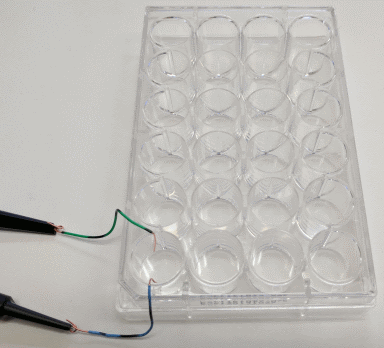
\includegraphics[scale=0.70]{electrophoresis}
	\caption{Electrode setup for investigating electrophoresis.}
	\label{fig:electroph}
\end{figure}

Now investigate how saline solutions 'screen' the charge on the glass beads, by determining their `effective' charge in the various solutions that you are asked to investigate in table~\ref{tab:lab7-vids}.

\begin{table}[ht]
	\centering
	\begin{tabular}{|c|c|c|}
	\hline 
	\textbf{Investigation} & \textbf{Video 1} & \textbf{Video 2} \\ 
	\hline 
	\textbf{A} & 2 um beads in DI & 2 um beads in LOW \\ 
	\hline 
	\textbf{B} & 2 um beads in DI & 2 um beads in HIGH \\ 
	\hline 
	\textbf{C} & 5 um beads in DI & 5 um beads in LOW \\ 
	\hline 
	\end{tabular}
	\caption{Videos. `DI' refers to De-Ionized water. `LOW' refers to a saline solution with 9 mg/L NaCl; `HIGH' refers to a saline solution with 90 mg/L NaCl. The viscosities of these solutions are almost identical: $9.0 \times 10^{-4}$ Pa s at 26 $^{\circ}$C.}
	\label{tab:lab7-vids}
\end{table} 

\paragraph*{Things you might consider including in your lab report:} In addition to the standard lab report, be sure to include a thorough discussion of both the qualitative and quantitative differences between the two solutions that you investigated.
Also discuss how you modeled the situation, how your model informed which forces you needed to consider, and what equation did it lead you to derive to calculate the charge of the glass beads in the fluid.
Discuss the ways in which the ideas explored here relate to biology and/or chemistry.
%Some other questions you may want to consider:
%\begin{itemize}
%\item 
%\item 
%\item 
%\end{itemize}